
\usepackage{tikz}
\usepackage[utf8]{inputenc}
\usepackage{amsmath}
\usepackage{amsfonts}
\usepackage{amssymb}
\usepackage{stackrel}
%\usepackage{kpfonts}
\usepackage{amssymb, amsmath, amsbsy} 
\usepackage{makeidx}
\usepackage{graphicx}
\usepackage{multicol}
\usepackage{changepage}
\usepackage{float}
\usepackage{cite}
\usepackage{lipsum}
\usepackage{pstricks, caption}
\usepackage{url}
\usepackage[spanish, es-tabla]{babel}
\usepackage[shortlabels]{enumitem}
\usepackage{longtable,multirow,booktabs}
\usepackage{rotating}
\usepackage{caption}
\usepackage{multirow, array}
\usepackage{anyfontsize}
\usepackage{fix-cm}
\usepackage{calligra}
\usepackage{mathptmx}
\usepackage{caption}
\usepackage{fancyvrb}
%\usepackage{esvect}
\usepackage{xargs}
\usepackage{subfigure} 
\usepackage {titletoc}
\usepackage[T1]{fontenc}
%\usepackage[hyphens]{url}
\usepackage[breaklinks,colorlinks=true,linkcolor=blue,citecolor=red, urlcolor=blue]{hyperref}
\usepackage{flushend}


\documentclass[13,twocolumn,letterpaper]{article}
    \usepackage[spanish,english]{babel}
    \usepackage[utf8x]{inputenc}
    \usepackage[T1]{fontenc}
    \usepackage[a4paper,top=3cm,bottom=2cm,left=3cm,right=3cm,marginparwidth=1.75cm]{geometry}
    \usepackage{amsmath}
    \usepackage[colorinlistoftodos]{todonotes}
    \usepackage[colorlinks=true, allcolors=blue]{hyperref}
    \usepackage{float}
    
    
 \spanishdecimal{.}
\renewcommand{\figurename}{\textbf{Figura}}
\renewcommand{\tablename}{\textbf{Tabla}}
\renewcommand{\refname}{Bibliografía}
\renewcommand{\abstractname}{\large\textbf{Resumen}}
\renewcommand{\contentsname}{Contenido}
\renewcommand{\partname}{Parte}
\renewcommand{\appendixname}{Apéndice}
\renewcommand{\sin}{sen}	
\newenvironment{Figure}{\par\medskip\noindent\minipage{\linewidth}}{\endminipage\par\medskip}

    
    \title{
    		%\vspace{-1in} 	
    		\usefont{OT1}{bch}{b}{n}
    		\normalfont \normalsize \textsc{INSTITUTO POLITÉCNICO NACIONAL \\ 
    		ESCUELA SUPERIOR DE FISICA Y MATEMATICAS \\
    		ACADEMIA DE FÍSICA EXPERIMENTAL} \\ 
    		FÍSICA IV: LABORATORIO DE ÓPTICA. \\[10pt]
    		\huge Práctica VIII :\\
  Polarización.\\
    }
    
    \usepackage{authblk}
    \author[0]{Alumno: Flores Rodriguez Jaziel David \\
    Boleta: 2014030429 \\
    Profesor: Dr. Janos Zsargo\\
    Grupo: 4FV2-B \\
            }
    \begin{document}
    
    \maketitle
   
    \selectlanguage{spanish}
    
    \section*{Resumen}
   Se estudió el efecto de la polarización en la luz, y se aprovecharon éstas propiedades para determinar tanto el ángulo de Brewster así como el índice de refracción de diferentes materiales, además se pudo obtener la ley de Malus	por el fenómeno de polarización por absorción selectiva mediante el uso de filtros polaroid.  \\\\	Palabras clave: \emph{ángulo de Brewster, ley de Malus, filtros polaroid}. \\ 



	\section*{Introducción}
		 La \textbf{polarizaci\'on electromagn\'etica} es una propiedad de las ondas que pueden oscilar con m\'as de una orientaci\'on. Esto se refiere normalmente a las llamadas ondas transversales, en particular se suele hablar de las ondas electromagn\'eticas, aunque tambi\'en se puede dar en ondas mec\'anicas transversales. En una onda electromagn\'etica, tanto el campo el\'ectrico y el campo magn\'etico son oscilantes, pero en diferentes direcciones; ambas perpendiculares entre sí y perpendiculares a la direcci\'on de propagaci\'on de la onda; por convenci\'on, el  plano de polarizaci\'on de la luz se refiere a la polarizaci\'on del campo el\'ectrico.
	La forma trazada sobre un plano fijo por un vector de campo el\'ectrico de una onda plana que pasa sobre \'el es una curva de Lissajous y puede utilizarse para describir el tipo de polarizaci\'on de la onda. Las siguientes figuras muestran algunos ejemplos de la variaci\'on del vector de campo el\'ectrico (azul) con el tiempo (el eje vertical), con sus componentes X y Y (roja/izquierda y verde/derecha), y la trayectoria trazada por la punta del vector en el plano (p\'urpura). Cada uno de los tres ejemplos corresponde a un tipo de polarización.
	\subsection*{Polarización por reflexión}
	{
		Al reflejarse un haz de luz no polarizado sobre una superficie, la luz reflejada sufre
		una polarización parcial de forma que el componente del campo eléctrico
		perpendicular al plano de incidencia (plano que contiene la dirección del rayo de
		incidencia y el vector normal a la superficie de incidencia) tiene mayor amplitud
		que el componente contenido en el plano de incidencia. Cuando la luz incide sobre una
		superficie no absorbente con un
		determinado ángulo, el componente del
		campo eléctrico paralelo al plano de
		incidencia no es reflejado. Este ángulo,
		conocido como ángulo de Brewster, en
		honor del físico británico David
		Brewster, se alcanza cuando el rayo
		reflejado es perpendicular al rayo
		refractado. La tangente del ángulo de
		Brewster es igual a la relación entre los
		índices de refracción del segundo y el
		primer medio. Además esto sucede
		cuando $\theta_{i}+\theta_{t}=90^{\circ}$ (figura \ref{fig:fig1}).\\
		\begin{figure}[h!]
			\centering
			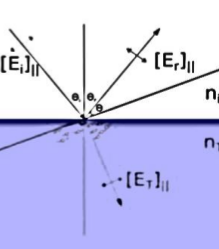
\includegraphics[width=0.7\linewidth]{fig1}
			\caption{}
			\label{fig:fig1}
		\end{figure}
		Usando la Ley de Snell
		\begin{equation}\label{ec1}
		n_{i}\sen\theta_{i}=n_{t}\sen\theta_{t}
		\end{equation}
		donde 
		\begin{equation}\label{ec2}
		\theta_{t}=90^{\circ}-\theta_{i}
		\end{equation}
		luego 
		\begin{equation}\label{ec3}
		\sen\theta_{t}=\sen(90^{\circ}-\theta_{i})=\cos\theta_{i}
		\end{equation}
		entonces sustituyendo (\ref{ec3}) en (\ref{ec1}) obtenemos 
		\begin{equation}\label{ec4}
		n_{i}\sen\theta_{i}=n_{t}\cos\theta_{i}
		\end{equation}
		De esta manera 
		\begin{equation}\label{ec5}
		\tan\theta_{i}=\left(\dfrac{n_{t}}{n_{i}}\right)
		\end{equation}
		Así el ángulo de Brewster está dado por:
		\begin{equation}\label{ec6}
		\theta_{i}=\tan^{-1}\left(\dfrac{n_{t}}{n_{i}}\right)
		\end{equation}
	}
	\subsection*{Intensidad de luz(Irradiancia)}
	{
		Se denomina vector de Poynting al vector cuyo módulo representa la intensidad
		instantánea de energía electromagnética que fluye a través de una unidad de área
		perpendicular a la dirección de propagación de la onda electromagnética, y cuyo
		sentido es el de propagación. Recibe su nombre del físico inglés John Henry
		Poynting. Se expresa mediante el símbolo \textbf{S}.\\
		El vector de Poynting puede definirse como el producto vectorial del campo
		eléctrico y el campo magnético, cuyo módulo es la intensidad de la onda:	
		\begin{equation}\label{ec7}
		\vec{S}=c^{2}\epsilon_{0}\vec{E}\times\vec{B}
		\end{equation}
		o bien 
		\begin{equation}\label{ec8}
		\vec{S}=\dfrac{1}{\mu}\vec{E}\times\vec{B}
		\end{equation}
		donde $\vec{E}$ y $\vec{B}$ representan el campo el\'ectrico y el campo de inducción magnética respectivamente siendo $\mu$ la permeabilidad magnética del medio. Su unidad en SI es el $vatio/m^{2}$.\\
		Dado que los campos eléctrico y magnético de una onda electromagnética oscilan
		con la frecuencia de la onda, la magnitud del vector de Poynting cambia en el
		tiempo. El promedio del vector de Poynting sobre un período muy superior al
		periodo de la onda es llamado irradiancia, I:
		\begin{equation}\label{ec9}
		I\equiv\langle\vec{S}\rangle
		\end{equation}
		La irradiancia representa el flujo de energía asociado a la radiación
		electromagnética en la dirección perpendicular a su dirección de propagación.
		Como puede verse, la intensidad de onda es proporcional a la amplitud del campo
		eléctrico, es decir:
		\begin{equation}\label{ec10}
		I_{0}\alpha E_{0}^{2}
		\end{equation}
		\begin{equation}\label{ec11}
		I\alpha E_{0}^{2}\cos\theta
		\end{equation}
		Como la constante de proporcionalidad es la misma se tiene que 
		\begin{equation}\label{ec12}
		I(\theta)=E_{0}^{2}\cos^{2}\theta
		\end{equation}
	}
\section*{Desarrollo experimental} 
se realizaron dos experimentos los cuales fueron los siguientes
\subsection*{Experimento 1 }
Éste consistió en determinar el índice de refracción de una sustancia utilizando el  sistema mostrado en la figura \ref{fig:fig2}.
\begin{figure}[h!]
	\centering
	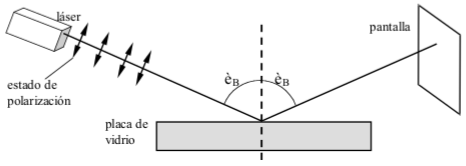
\includegraphics[width=0.7\linewidth]{fig2}
	\caption[Figura 1]{Sistema utilizado en el experimento 1.}
	\label{fig:fig2}
\end{figure}
\\Aquí se hará uso de la propiedad de la polarización y del ángulo de Brewster, con la particularidad de que en este caso $n_{i}=1$, por tanto, sustituyendo $n_{i}=1$ en \ref{ec5} se tiene que
\begin{equation}\label{ec13}
	\tan\theta_{i}=n_{t}
\end{equation}
Para obtener el ángulo de Brewster se desplazó el láser por la circunferencia, el
haz se era reflejado por la sustancia en el recipiente e incidía sobre la pantalla, el
punto donde éste desaparecía (se deja de ver) es cuando el ángulo incidente es
igual al ángulo de Brewster, así que se anotaba el ángulo medido.
\subsection*{Experimento 2}
En este caso utilizamos el  sistema de la figura \ref{fig:fig3}.
\begin{figure}[h!]
	\centering
	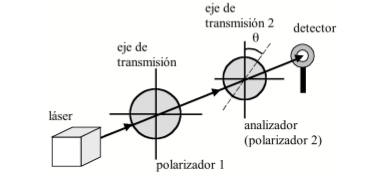
\includegraphics[width=0.7\linewidth]{fig3}
	\caption[Figura 1]{Sistema utilizado en el experimento 2.}
	\label{fig:fig3}
\end{figure}
Con un medidor de intensidad registramos la intensidad que llegaba al detector
cuando variábamos el ángulo de desfase entre los polarizadores, dejando fijo el
ángulo del polarizador 1 con respecto al láser.
\section*{Datos y resultados obtenidos}
\subsection*{Experimento 1}
En el experimento 1 se traro de determinar el ángulo de Brewster
los datos que se obtuvieron son los siguientes datos donde $\theta_{h_{2}o}$, $\theta_{gli}$ y $\theta_{acr}$ son los ángulos obtenidos para el agua, la glicerina y el acrílico respectivamente. 
\begin{table}[htb]
	\centering
	\begin{tabular}{cccc}
		N & $\theta_{h_{2}o}$ $(^{\circ})$ & $\theta_{gli}$ $(^{\circ})$ & $\theta_{acr}$ $(^{\circ})$  \\ \midrule
		1  &  53 	& 55 	&	55  \\
		2  &  52 	& 54 	&	56 \\
		3  &  52.5 	& 54.5	&	55.5  \\
		4  &  53.5 	& 55.5 	&	55.5  \\ 
		&&&\\
		Promedio  & 52.75  & 54.75 & 55.5 \\\hline
	\end{tabular}
	\caption{Datos obtenidos en el experimento 1: Determinación del ángulo de Brewster} \label{tabla1}
\end{table}
\\Utilizando la ecuación \ref{ec13} se obtuvo lo siguiente:\\
Para el agua 
\begin{equation}
tan\theta_{h_{2}o}=n_{h_{2}o} \implies tan(52.75)=1.3150
\end{equation}
Para la glicerina:
\begin{equation}
tan\theta_{gli}=n_{gli} \implies tan(54.75)=1.4149
\end{equation}
Para el acrílico
\begin{equation}
tan\theta_{acr}=n_{acr} \implies tan(55.5)=1.4550
\end{equation}
\\Así pues los resultados para este experimento  fueron
$$tan\theta_{h_{2}o}=1.3150$$
$$tan\theta_{gli}=1.4149$$
$$tan\theta_{acr}=1.4550$$
Los indices de refracción teóricos para estos materiales son:
$$tan\theta_{h_{2}o}=1.33$$
$$tan\theta_{gli}=1.47$$
$$tan\theta_{acr}=1.49$$
Los porcentajes de error obtenidos fueron:\\
Para el agua
$$\%e=\dfrac{|1.3150 - 1.33|}{1.3150}\times 100=1.1406 \%$$
Para la glicerina
$$\%e=\dfrac{|1.4149 - 1.47|}{1.4149}\times 100=3.8819 \%$$
Para el acrílico
$$\%e=\dfrac{|1.4550 - 1.49|}{1.4550}\times 100=2.5054 \%$$
\subsection{Experimento 2}
Para el segundo experimento considerando las medidas tomadas y así llenamos
la  tabla \ref{tabla2}.
\begin{table}[htb]
	\centering
	\begin{tabular}{ccccc}
		N & $\theta$ & $\cos\theta$ & $\cos^{2}\theta$  & $I(\theta)$ \\ \midrule
		1  & 0 	& 1 	 &	1	 	& 116.4	 \\
		2  & 20 & 0.94 	 & 0.8836 	& 102.6	 \\
		3  & 40 & 0.77	 & 0.5929	& 66.4	 \\
		4  & 60 &  0.5	 & 0.25		& 24.1	 \\
		5  & 75 & 0.5588 & 0.0669   & 4.8    \\
		6  & 80 & 0.1736 & 0.0301   & 1.5	 \\\hline
	\end{tabular}
	\caption{Datos obtenidos en el experimento 2} \label{tabla2}
\end{table}
\newpage Y con estos datos generamos la grafica de $I(\theta) \;vs\;\cos^{2}\theta$ la cual es la siguiente
\begin{figure}[h!]
	\centering
	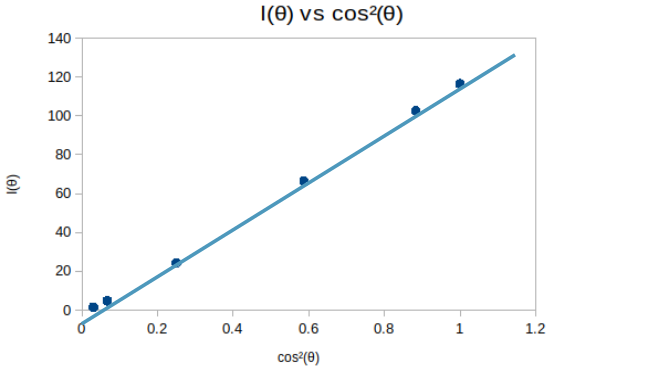
\includegraphics[width=1.2\linewidth]{fig4}
	\caption[Figura 1]{Ajuste $I(\theta)\;vs\;\cos^{2}(\theta)$}
	\label{fig:fig4}
\end{figure}
\\La ecuaci\'on de ajuste que se obtuvo fue la siguiente:
\begin{equation}
	I(\theta)=119.58\cos^{2}(\theta)-3.6372
\end{equation}
\section*{Conclusiones}
En el primer experimento se obtuvieron errores porcentuales muy bajos por lo que las mediciones obtenidas fueron buenas, lo cual demuestra que si se cumple lo visto en teoría.\\
Finalmente, para la segunda parte se obtuvo una gráfica bastante parecida a la
que la Ley de Malus describe, claramente mientras haya un ángulo de desfase
mayor la intensidad de luz disminuye, lo que nos dice que existe una mayor
polarización.
\nocite{Hecht}\nocite{Rossi}\nocite{Sears}\nocite{Born}\nocite{Tipler}\nocite{Feynman}\nocite{Res}
\bibliography{miBiblio.bib}
\bibliographystyle{plain}
\end{document}